\documentclass[11pt,letterpaper]{article}
\usepackage[margin=0.88in]{geometry}
\usepackage[T1]{fontenc}
\usepackage{lmodern,microtype}
\usepackage{amsmath,amssymb,amsthm,mathtools}
\usepackage{booktabs,longtable,array,tabularx}
\usepackage{graphicx,xcolor,pdflscape}
\usepackage{enumitem,listings}
\usepackage[unicode,colorlinks=true,linkcolor=teal!55!black,urlcolor=teal!55!black,citecolor=teal!55!black]{hyperref}
\usepackage{fancyhdr}
\pagestyle{fancy}\fancyhf{}
\fancyhead[L]{\small Largest sections of the Platonic solids}
\fancyhead[R]{\small Constructive arithmetic proof}
\fancyfoot[C]{\thepage}
\setlength{\headheight}{14pt}
\setlength{\emergencystretch}{3em}
\setlist{topsep=4pt,itemsep=3pt}
\newtheorem{theorem}{Theorem}[section]
\newtheorem{lemma}[theorem]{Lemma}
\newtheorem{proposition}[theorem]{Proposition}
\theoremstyle{definition}\newtheorem{definition}[theorem]{Definition}
\newcommand{\conv}{\operatorname{conv}}
\newcommand{\Area}{\operatorname{Area}}
\newcommand{\ipra}{\mathrm{iPRA}}
\newcommand{\QQ}{\mathbb Q}
\newcommand{\RR}{\mathbb R}
\newcommand{\llbracket}{[\![}
\newcommand{\rrbracket}{]\!]}
\lstset{basicstyle=\ttfamily\small,breaklines=true,columns=fullflexible,frame=single,
  backgroundcolor=\color{gray!4},rulecolor=\color{gray!25},showstringspaces=false}
\hypersetup{pdftitle={Largest planar sections of the five Platonic solids},
 pdfauthor={Constructive geometry research report}}
\title{\textbf{Largest planar sections\\of the five Platonic solids}\\[5pt]
 \large Explicit optimizers, exact certificates, and an iPRA formalization plan}
\author{}
\date{19 November 2026}
\begin{document}
\maketitle
\begin{abstract}
We find a largest planar section of each Platonic solid, give its equation,
vertices, shape, and exact area, and prove a global upper bound. The
tetrahedral, cubical, and octahedral bounds have short elementary algebraic
proofs. The icosahedral and dodecahedral bounds reduce to two and three
explicit cones of normals and finite positive-coefficient polynomial
certificates. All 283 nonzero certificate coefficients are printed in the
appendices and supplied in machine-readable form. An exact finite
trapezoid construction reduces affine sections of centrally symmetric
solids to central sections. The resulting proof uses only finite geometry,
ordered quadratic-field arithmetic, and primitive recursive operations.
We state its first-order arithmetical interpretation precisely and give a
Lean outline directed at ProveIt's actual \texttt{Prf PRAAx} interface.
The Python certificates have been executed; the Lean outline is not a
completed or kernel-checked formalization of the main theorem.
\end{abstract}

\section{Answer, normalization, and conventions}
Let $a>0$ be the edge length of the solid, and put
$\varphi=(1+\sqrt5)/2$. The answer is as follows.
\begin{center}
\renewcommand{\arraystretch}{1.4}
\begin{tabular}{@{}lll@{}}
\toprule
Solid & Shape of an attaining section & Maximum area\\
\midrule
Tetrahedron & Equilateral face & $\displaystyle\frac{\sqrt3}{4}a^2$\\
Cube & Rectangle, sides $a,\sqrt2a$ & $\sqrt2a^2$\\
Octahedron & Square, side $a$ & $a^2$\\
Icosahedron & Centrally symmetric hexagon & $\displaystyle\frac{2+\sqrt5}{2}a^2$\\
Dodecahedron & Regular decagon, side $\varphi a/2$ &
 $\displaystyle\frac5{16}\sqrt{130+58\sqrt5}\,a^2$\\
\bottomrule
\end{tabular}
\end{center}
The corresponding numerical coefficients of $a^2$ are, respectively,
$0.4330127019$, $1.4142135624$, $1$, $2.1180339887$, and
$5.0359250668$. The hexagon is not regular: its two opposite long sides
have length $a$, and its other four sides have length $\sqrt3a/2$.

\paragraph{Meaning of section.}
A section is the intersection of the closed solid with an affine plane;
supporting planes are allowed. This convention is essential for the
tetrahedron, whose largest section is one of its faces. If the plane must
meet the interior of the tetrahedron, the displayed value is the supremum
and is not attained. The other four displayed planes meet the interior.
We seek one maximizing plane for each solid, not a classification of all
possible translated equality cases.

\subsection{Coordinate models and equations}
The following unscaled models keep every coordinate in
$\QQ(\varphi)$. Each independent $\pm$ sign ranges over both choices.
\begin{align*}
T={}&\conv\{(1,1,1),(1,-1,-1),(-1,1,-1),(-1,-1,1)\},\\
C={}&[-1,1]^3,\\
O={}&\conv\{\pm e_1,\pm e_2,\pm e_3\},\\
I={}&\conv\{(0,\pm1,\pm\varphi),(\pm1,\pm\varphi,0),
                       (\pm\varphi,0,\pm1)\},\\
D={}&\conv\{(\pm1,\pm1,\pm1),(0,\pm\varphi^{-1},\pm\varphi),\\
 &\hspace{53mm}(\pm\varphi^{-1},\pm\varphi,0),
                       (\pm\varphi,0,\pm\varphi^{-1})\}.
\end{align*}
Here $e_j$ are the coordinate unit vectors and
$\varphi^{-1}=\varphi-1$. The scale factors taking these models to edge
length $a$, and the desired planes in the unscaled models, are
\begin{center}
\renewcommand{\arraystretch}{1.3}
\begin{tabular}{@{}llll@{}}
\toprule
Model & Raw edge length & Scale factor & Maximizing plane\\
\midrule
$T$ & $2\sqrt2$ & $a/(2\sqrt2)$ & $x+y+z=-1$\\
$C$ & $2$ & $a/2$ & $x+y=0$\\
$O$ & $\sqrt2$ & $a/\sqrt2$ & $z=0$\\
$I$ & $2$ & $a/2$ & $z=0$\\
$D$ & $2/\varphi$ & $a\varphi/2$ & $\varphi y+z=0$\\
\bottomrule
\end{tabular}
\end{center}
Thus, in the scaled physical coordinates, the tetrahedral equation is
$x+y+z=-a/(2\sqrt2)$; the four homogeneous plane equations stay the same.
Multiplying every listed section vertex below by its scale factor gives
the coordinates for any requested edge length.

\paragraph{Relation to existing results.}
The maximizing values and orientations agree with the computations of
Brandenburg, De Loera, and Meroni, Example 5.2 and Table 3 of
\cite{BDM}. Their paper provides a general framework for slicing
polytopes. Here the global bounds are supplied by explicit finite
identities, coefficient lists, and independently executable checks. No
call to a numerical optimizer is used as a premise of the proof.

\begin{landscape}
\begin{figure}[p]
\centering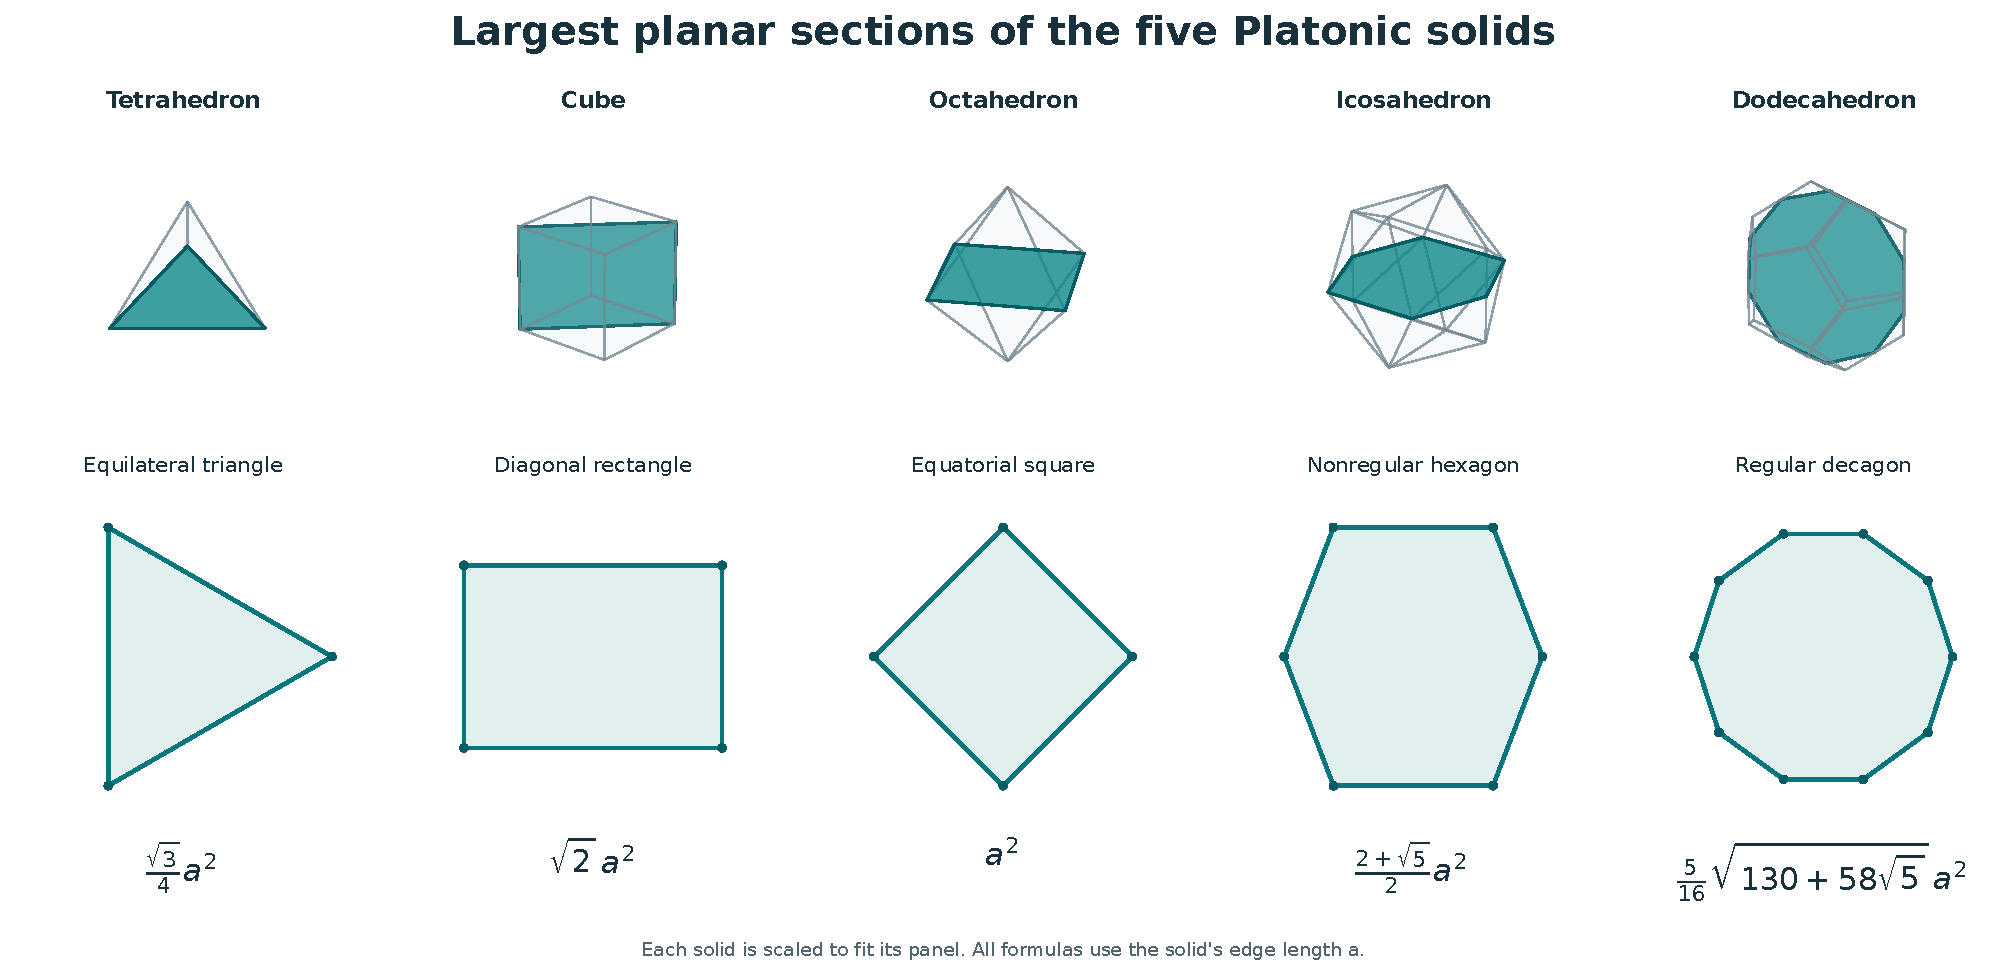
\includegraphics[width=\linewidth]{figures/maximal_sections.pdf}
\caption{The five attaining sections. The drawings use the exact vertices
given in the text. Floating point is used only to render the illustration;
all geometric and certificate checks use exact arithmetic.}
\end{figure}
\end{landscape}

\tableofcontents
\clearpage

\section{Finite geometric definitions and elementary tools}
\label{sec:finitegeometry}
\subsection{Solids, planes, and polygons}
For a finite list of points $v_0,\ldots,v_{r-1}$, their convex hull is
the set of sums $\sum_i\lambda_i v_i$ with $\lambda_i\ge0$ and
$\sum_i\lambda_i=1$. A plane is
\[
 H(n,t)=\{x:n\cdot x=t\},\qquad n\ne0.
\]
The input $(n,t)$ is unchanged geometrically by multiplying it by a
nonzero scalar. A convex polygon is specified by its boundary vertices
$q_0,\ldots,q_{m-1}$ in cyclic order. Repeated boundary vertices are
permitted and contribute zero edges. Empty polygons, points, and
segments have area zero.

The section vertices are the original vertices lying on the plane,
together with the intersections of the plane and the crossed polytope
edges. For an edge $[v_i,v_j]$, put $h_i=n\cdot v_i-t$. If $h_i,h_j$
have opposite signs, its intersection is
\begin{equation}
 q_{ij}=\frac{h_i v_j-h_j v_i}{h_i-h_j}.             \label{eq:edge}
\end{equation}
If the whole edge lies in the plane, insert its endpoints instead.
All these decisions are finite sign tests for arithmetic input data.

To justify completeness, let a section vertex lie in the relative
interior of a face of the original polytope of dimension at least two.
Intersecting that face's affine span with the plane leaves a line
through the point, unless the plane contains the face, in which case
there is again such a line. A sufficiently small segment of this line
lies in the face, contradicting extremality in the section. Thus a
section vertex lies on an original edge or is an original vertex.
This reasoning can be expressed by the finitely many supporting
inequalities and linear nullspaces; it needs no infinite separation
theorem. The convex hull of the resulting finite point list is the
whole section.

\subsection{Squared area without square roots}
The vector shoelace formula gives
\begin{equation}
 W(Q)=\frac12\sum_{i=0}^{m-1}q_i\times q_{i+1},
 \qquad \Area(Q)^2=W(Q)\cdot W(Q),                 \label{eq:area}
\end{equation}
with indices taken modulo $m$. To prove it, triangulate from a point
of the polygon. The oriented triangle vectors add, and the terms
involving that point telescope. All vectors are parallel and have
the same orientation, so the norm of their sum is the sum of their
areas. This also proves finite additivity. Alternatively, dropping
any coordinate $j$ with $n_j\ne0$ gives a planar shoelace formula;
the conversion factor is $\|n\|/|n_j|$.

For arithmetic purposes, (\ref{eq:area}) is the definition of the
squared-area output. It lies in the original coordinate field even
when the positive area itself requires a further square root.
All sharp comparisons can therefore be checked by ordered-field
arithmetic in $\QQ(\varphi)$.

\subsection{Weighted vector bounds}
The norm inequalities used below have polynomial certificates. If
$\lambda_i\ge0$ and $s=\sum_i\lambda_i$, then
\begin{equation}
 s\sum_i\lambda_i\|v_i\|^2-
   \left\|\sum_i\lambda_i v_i\right\|^2
 =\sum_{i<j}\lambda_i\lambda_j\|v_i-v_j\|^2\ge0.
                                                               \label{eq:variance}
\end{equation}
Consequently, if $s\le1$ and every $\|v_i\|^2\le M^2$, then
$\|\sum_i\lambda_i v_i\|^2\le M^2$.
Thus any application below of the triangle inequality to a weighted
sum of face vectors can be replaced by a finite polynomial identity.
This avoids an implicit appeal to a complete normed space.

\subsection{Checking the coordinate models}
The programs enumerate supporting facets and edge incidences exactly.
The counts are $(V,E,F)=(4,6,4),(8,12,6),(6,12,8),(12,30,20),
(20,30,12)$ in the order $T,C,O,I,D$. All triangular facets are
equilateral, all cubical facets are squares, and the dodecahedral
facets are regular pentagons. In the latter model, the outward
normals are $(0,\pm\varphi,\pm1),(\pm1,0,\pm\varphi),
(\pm\varphi,\pm1,0)$, with common support constant $\varphi^2$;
their edge squares are $8-4\varphi$ and diagonal squares are $4$.
These finite supporting-plane checks identify the standard regular
solids and verify that no unlisted facet is used in a section formula.

\section{An exact central-section reduction by finite trapezoids}
The four centrally symmetric Platonic solids admit a common reduction:
for each plane orientation, a central section has at least as much area
as every parallel section.  In the present three-dimensional problem
this needs only a finite polygon construction.  A general
Brunn--Minkowski theorem, a limiting argument, and integration are
unnecessary.

\subsection{The planar finite construction}
Let $S$ be a convex polygon with at most $m$ vertices.  We prove
\[
 \operatorname{area}\bigl((S-S)/2\bigr)
 \ge \operatorname{area}(S).
\]
An empty polygon or a polygon of area zero causes no difficulty: its
area is zero, and the desired inequality follows from nonnegativity.
For completeness the construction below also handles a nonvertical
segment.  Let the horizontal projection be $[a,b]$.  If $a=b$, the
polygon lies on a vertical line and has area zero.  Assume $a<b$.

Write its vertical fibers as $[\ell(x),u(x)]$ for $a\le x\le b$.
The functions $\ell$ and $u$ are respectively convex and concave,
continuous piecewise-affine functions.  Their breakpoints occur among
the horizontal coordinates of the original polygon vertices.  This
follows directly by reading the lower and upper boundary chains of a
convex polygon.  Put $f(x)=u(x)-\ell(x)\ge0$, and let
\[
 c=(a+b)/2,\qquad \rho(x)=a+b-x.
\]
Construct a new polygon $W$ whose fiber over horizontal coordinate
$x-c$ has endpoints
\[
 L(x)=\frac{\ell(x)-u(\rho(x))}{2},\qquad
 H(x)=\frac{u(x)-\ell(\rho(x))}{2}.
\]
Their difference is
\[
 h(x)=H(x)-L(x)
      =\frac{f(x)+f(\rho(x))}{2}\ge0.                 \tag{CS1}
\]
The lower function $L$ is convex, and the upper function $H$ is
concave: composition with the affine reflection $\rho$ preserves
convexity or concavity, and taking the negative interchanges them.
Thus the region between these boundary chains is a convex polygon.

Its containment is also explicit.  The point $(x-c,L(x))$ is the
half-difference of $(x,\ell(x))\in S$ and
$(\rho(x),u(\rho(x)))\in S$, while $(x-c,H(x))$ is the
half-difference of $(x,u(x))\in S$ and
$(\rho(x),\ell(\rho(x)))\in S$.  Indeed their first coordinates
are $(x-\rho(x))/2=x-c$.  Since $(S-S)/2$ is convex, it contains the
whole segment between these endpoints and consequently all of $W$.
Equivalently, it suffices to check the finitely many boundary vertices
of $W$ and then take their convex hull.

\subsection{Exact equality of areas}
Take the distinct horizontal vertex coordinates of $S$, adjoin their
reflections under $\rho$, and sort the resulting finite set:
\[
 a=x_0<x_1<\cdots<x_r=b.
\]
There are at most $2m$ distinct breakpoints, so $r\le2m-1$.
The list is reflection invariant:
\[
 x_i+x_{r-i}=a+b \qquad(0\le i\le r).
\]
Between consecutive breakpoints all four functions
$\ell,u,\ell\circ\rho,u\circ\rho$ are affine.  Hence $S$ is the
union, with disjoint interiors, of its vertical trapezoids over these
intervals.  If $f_i=f(x_i)$ and $\Delta_i=x_{i+1}-x_i$, their areas are
\[
 T_i=\frac{\Delta_i}{2}(f_i+f_{i+1}),\qquad
 \operatorname{area}(S)=\sum_{i=0}^{r-1}T_i.          \tag{CS2}
\]
A zero endpoint height merely gives a triangle.  The trapezoid formula
follows by splitting into triangles or by a four-vertex shoelace
calculation; finite area additivity gives the second equality.

The corresponding slab of $W$ runs from $x_i-c$ to $x_{i+1}-c$.
Its horizontal width is still exactly $\Delta_i$: the coordinate map
$x\mapsto x-c$ is a translation, not a dilation.  From (CS1), its
endpoint heights are $(f_i+f_{r-i})/2$ and
$(f_{i+1}+f_{r-i-1})/2$.  Its area is therefore
\[
 \begin{split}
 U_i
 &=\frac{\Delta_i}{4}
      (f_i+f_{i+1}+f_{r-i}+f_{r-i-1})\\
 &=\frac12 T_i+\frac12 T_{r-i-1},
 \end{split}                                       \tag{CS3}
\]
because reflection gives $\Delta_i=\Delta_{r-i-1}$.
Summing (CS3), the reversed finite index list is a permutation of the
original list, and we obtain
\[
 \operatorname{area}(W)
 =\sum_{i=0}^{r-1}U_i
 =\frac12\sum_{i=0}^{r-1}T_i
  +\frac12\sum_{i=0}^{r-1}T_{r-i-1}
 =\operatorname{area}(S).                           \tag{CS4}
\]
As $W\subseteq(S-S)/2$, area monotonicity proves the asserted inequality.
For polygons, this monotonicity is itself a finite fact: refine by the
finitely many vertical breakpoints of both polygons, compare the
nonnegative fiber heights at the endpoints, and use the same trapezoid
formula.  No measure-theoretic premise is needed.

\subsection{Application to an affine section of a symmetric polytope}
Suppose $K=-K$ is a convex three-dimensional polytope, and write
\[
 S=K\cap\{n\cdot x=t\},\qquad
 S_0=K\cap\{n\cdot x=0\},\qquad n\ne0.
\]
For $p,q\in S$, convexity and central symmetry put $(p-q)/2$ in $K$,
and $n\cdot((p-q)/2)=0$.  Consequently
\[
 (S-S)/2\subseteq S_0.
\]
Identify the two parallel planes by translation.  The finite planar
construction gives a polygon $W\subseteq S_0$ having exactly the area
of $S$.  Hence
\[
 \boxed{\ \operatorname{area}(S)\le\operatorname{area}(S_0).\ }
\]
This argument includes supporting-plane sections, so no continuity at
a supporting face is being assumed.

\subsection{Arithmetic coordinates and the iPRA invariant}
For arithmetic inputs, an orthonormal frame is unnecessary.  Drop any
coordinate $j$ for which $n_j\ne0$.  The remaining two coordinates
provide an injective affine chart for both parallel planes; their
Euclidean areas have the same positive conversion factor
$\|n\|/|n_j|$.  Apply the preceding construction and area comparison to
the projected polygons.  All breakpoints, fiber endpoints, translated
coordinates, and trapezoid areas belong to the original ordered
arithmetic field.  The common positive conversion factor cancels.

The construction uses at most $2m$ distinct breakpoints and at most
$4m$ listed boundary vertices for $W$.  Sorting, merging, boundary-chain
traversal, and evaluating affine functions are primitive recursive.
A quantifier-free induction invariant for the summation loop is
\[
 2\sum_{i<k}U_i
   =\sum_{i<k}T_i+\sum_{i<k}T_{r-i-1}
 \qquad(0\le k\le r),                              \tag{CS5}
\]
where all sums are defined primitive-recursively on the finite lists.
The step is exactly (CS3); at $k=r$, reversing the finite sum gives
(CS4).  The convexity and containment checks are finite endpoint
inequalities and arithmetic midpoint identities.  This supplies a
direct iPRA proof of the central-section reduction for coded polygons,
without any excluded-middle decision about arbitrary real inputs or
any unbounded search.

\section{Tetrahedron: the largest-face bound}
The following elementary argument works for every nondegenerate tetrahedron,
not only a regular one.  For three points define the oriented area vector by
\[
 F(P,Q,R)=\frac12(Q-P)\mathbin\times(R-P).
\]
Its norm is the area of the triangle.  This vector is affine in each of
its three arguments separately, as is clear from
$2F(P,Q,R)=P\times Q+Q\times R+R\times P$.
Consequently, if $P,Q,R$ are convex combinations of the four vertices,
then $F(P,Q,R)$ is a convex combination of the $4^3=64$ corresponding
vertex-triangle vectors.  The norm of each of those vectors is at most
$M$, the largest face area.  The triangle inequality therefore proves
that every triangle contained in the tetrahedron has area at most $M$.

It remains to consider a quadrilateral section.  Label the vertices
$A,B$ on one side and $C,D$ on the other, with respective positive
signed heights $a,b,-c,-d$.  Translate so that $A=0$, and put
$B=u,C=v,D=w$.  The vertices of the section in their cyclic order are
\[
 P=\alpha v,\quad Q=\beta w,\quad
 R=(1-\gamma)u+\gamma w,\quad
 S=(1-\delta)u+\delta v,
\]
where
\[
 \alpha=\frac a{a+c},\qquad \beta=\frac a{a+d},\qquad
 \gamma=\frac b{b+d},\qquad \delta=\frac b{b+c}.
\]
Set
\[
 E_1=\frac12u\times v,\quad E_2=-\frac12u\times w,
 \quad E_3=\frac12v\times w,\quad E_4=-E_1-E_2-E_3.
\]
These are signed face-area vectors, so $\lVert E_i\rVert\le M$.
The quadrilateral area vector is
\[
 G=\frac12(R-P)\times(S-Q)=pE_1+qE_2+rE_3,
\]
with
\begin{align*}
 p&=\alpha+\delta-\alpha\delta-\gamma\delta,\\
 q&=\beta+\gamma-\beta\gamma-\gamma\delta,\\
 r&=\alpha\beta-\gamma\delta.
\end{align*}
The four numbers $p,q,p-r,q-r$ are nonnegative.  For example,
\[
 p=\alpha(1-\delta)+\delta(1-\gamma),\qquad
 p-r=\alpha(1-\beta)+\delta(1-\alpha),
\]
and the two analogous formulas give the claim for $q,q-r$.
If $r\le0$, apply the triangle inequality to $G$ as displayed.
If $r\ge0$, instead use
\[
 G=(p-r)E_1+(q-r)E_2-rE_4.
\]
In both cases,
\[
 \lVert G\rVert\le(p+q-r)M.
\]
Finally the exact slack identity is
\begin{align*}
 1-(p+q-r)
 &=(\alpha+\gamma-1)(\beta+\delta-1)\\
 &=\frac{(ab-cd)^2}{(a+c)(a+d)(b+c)(b+d)}\ge0.
\end{align*}
This proves the desired bound.  Sections with a vertex of the tetrahedron
on the cutting plane are triangles or degenerate quadrilaterals.  In
the latter case the same argument holds with nonnegative heights,
provided the four displayed denominators are positive; if a denominator
vanishes, the plane contains that entire edge, and the section is a
triangle.  Thus no limiting argument is needed.

For the regular model
\[
 T=\operatorname{conv}\{(1,1,1),(1,-1,-1),(-1,1,-1),(-1,-1,1)\},
\]
the edge length is $2\sqrt2$.  The plane $x+y+z=-1$ gives a face of
area $2\sqrt3$.  With edge length $s$ the maximum is
$\sqrt3\,s^2/4$.
Here a planar section includes the intersection with a supporting
plane.  If one requires the plane to meet the interior of $T$, this
number is only a supremum: every genuine triangular or quadrilateral
cut has strictly smaller area.  In the quadrilateral argument this
follows from the strict triangle inequality for two nonparallel,
nonzero face-area vectors; for a triangle the affine expansion gives
equality only for a complete face.

\section{Cube: an elementary central-section bound}
Let $C=[-1,1]^3$.  Assume the separately proved central-section
dominance lemma for centrally symmetric convex polytopes.  Sign changes
and permutations of coordinates reduce the normal to
$a\ge b\ge c\ge0$, with $a>0$.  Put $x=b/a$, $y=c/a$.
The orthogonal graph of the central section over the $yz$ square is
\[
 X=-xY-yZ,\qquad |Y|,|Z|\le1,\quad |xY+yZ|\le1.
\]
Area on this graph equals projected area times
$\sqrt{1+x^2+y^2}$.

If $x+y\le1$, there is no truncation, and the area is
\[
 A=4\sqrt{1+x^2+y^2}\le4\sqrt2,
\]
because $x^2+y^2\le(x+y)^2\le1$.

If $x+y>1$, let $r=x+y-1\in(0,1]$.  Here $x,y>0$.
Exactly two opposite corners are removed from the projected square;
each removed right triangle has legs $r/x,r/y$.  Thus
\[
 \frac A4=\sqrt{1+x^2+y^2}\left(1-\frac{r^2}{4xy}\right).
\]
The elementary inequalities
\[
 x^2+y^2\le1+r^2,\qquad 4xy\le(1+r)^2
\]
follow respectively from $(1-x)(1-y)\ge0$ and $(x-y)^2\ge0$.
Hence
\[
 \frac A4\le\sqrt{2+r^2}\frac{1+2r}{(1+r)^2}\le\sqrt2.
\]
The last step is justified by the explicit polynomial identity
\[
 2(1+r)^4-(2+r^2)(1+2r)^2
 =r^2(3+4r-2r^2)
 =r^2\bigl(3+2r+2r(1-r)\bigr)\ge0.
\]
All factors being squared or multiplied are nonnegative.
Equality is achieved at $(x,y)=(1,0)$, i.e. $X+Y=0$.
The section is the rectangle with vertices
$(1,-1,1),(1,-1,-1),(-1,1,-1),(-1,1,1)$,
with side lengths $2,2\sqrt2$ and area $4\sqrt2$.
At edge length $s$ the maximum is $\sqrt2\,s^2$.

\section{Octahedron: an all-positive polynomial certificate}
Let $O=\{(X,Y,Z):|X|+|Y|+|Z|\le1\}$, with edge length $\sqrt2$.
Again use central-section dominance.  Coordinate symmetries reduce a
nonzero normal to $(a,b,c)$ with $a,b,c\ge0$ and $a>0$.
If $b=c=0$, the section is the square $X=0$, of area $2$.
Otherwise $D=(a+b)(a+c)(b+c)>0$, and its vertices, allowing duplicates
when a coefficient vanishes, are
\[
 P=\frac{(b,-a,0)}{a+b},\qquad
 Q=\frac{(c,0,-a)}{a+c},\qquad
 R=\frac{(0,c,-b)}{b+c},\qquad -P,-Q,-R.
\]
They occur in the listed cyclic order.  The shoelace area vector is
\[
 P\times Q+Q\times R-R\times P
 =\frac{2(ab+ac+bc)}D(a,b,c).
\]
Consequently
\[
 A=\frac{2\sqrt{a^2+b^2+c^2}(ab+ac+bc)}D\le2,
\]
where the inequality follows by squaring and using
\begin{align*}
 D^2-(a^2+b^2+c^2)(ab+ac+bc)^2
 ={}&2(a^3b^3+a^3c^3+b^3c^3)\\
 &+4abc(a^2b+a^2c+ab^2+ac^2+b^2c+bc^2)\\
 &+7a^2b^2c^2\ge0.
\end{align*}
Every monomial has a nonnegative coefficient.  If at least two normal
coordinates are positive, the difference is strictly positive, so the
only maximizing central planes are the coordinate planes.
For example $Z=0$ gives the square with vertices
$(1,0,0),(0,1,0),(-1,0,0),(0,-1,0)$.
Scaling to edge length $s$ gives maximum area $s^2$.

\section{Arithmetic and formalization notes}
All inequalities above have fixed finite algebraic proofs over ordered
fields.  The displayed slack identities are checked by
\texttt{verify\_small\_solids.py}; the checker is supplementary evidence,
and the identities themselves are visible certificates.
For iPRA, integer and rational arithmetic are primitive recursive;
sign cases are decidable for encoded rationals or fixed-degree real
algebraic coordinates.  The operations and loops have fixed finite
bounds.  One must separately supply the representation and error
control for arbitrary constructive plane normals, as in the common
framework, rather than assume that arbitrary real-number sign tests
are decidable.  Square roots in the Euclidean area formulas can be
replaced throughout the upper-bound verification by nonnegative squared
areas.  In Lean, the polynomial identities are \texttt{ring}; their
nonnegativity uses \texttt{positivity} and \texttt{nlinarith} after the
explicit denominator-positivity lemmas.  The geometric bridge uses
finite convex combinations, cross products, and cyclic polygon area
vectors; it does not need an unbounded search or an existence theorem
for a maximizing plane.

The generic tetrahedron largest-face theorem is historically recorded
in M. S. Klamkin, ``Largest Cross-Section of a Tetrahedron'',
\emph{American Mathematical Monthly} 82 (1975), p.~661, solution to
Problem E~1298, pointing back to Problem~5006 (1962--1963).
An author-hosted collected reprint is at
\url{https://carmamaths.org/resources/jon/Preprints/Books/Klamkin/komplete.pdf}.
The proof given here is complete independently of that reference.

\section{The icosahedron: an exact global certificate}
Put $\varphi=(1+\sqrt5)/2$ and let $I$ be the convex hull of
\[
 (0,\pm1,\pm\varphi),\qquad(\pm1,\pm\varphi,0),\qquad
 (\pm\varphi,0,\pm1).
\]
Its edge length is $2$. A largest section is $I\cap\{z=0\}$. In cyclic
order its vertices are
\[
 (\varphi,0,0),\ (1,\varphi,0),\ (-1,\varphi,0),\
 (-\varphi,0,0),\ (-1,-\varphi,0),\ (1,-\varphi,0).
\]
Thus it is a centrally symmetric, nonregular hexagon. Two opposite sides
have length $2$, and the other four sides have length $\sqrt3$. Its area is
\[
 M=2\varphi(\varphi+1)=2\varphi^3=4+2\sqrt5.
\]
For edge length $s$, the answer is therefore
$\frac{2+\sqrt5}{2}s^2$.

\subsection{A fundamental cone without an assumption about symmetric optima}
The reflections in $x=0$, $y=0$, and
$z=\varphi^2x+\varphi y$ all permute the twelve vertices. For the last one,
use the normal $m=(-\varphi^2,-\varphi,1)$, with
$m\cdot m=4\varphi^2$, and the formula
$R_m(v)=v-2(v\cdot m)m/(m\cdot m)$.
The group they generate is finite: its action on the twelve vertices is
faithful, since those vertices span space. For any nonzero normal $n$,
choose from its finite orbit a vector maximizing its scalar product with
$h=(1,1,10)$. Since $h$ has positive scalar product with each inward
wall normal, reflection in a violated wall would increase that scalar
product. Consequently the chosen vector lies in
\[
 C=\{(x,y,z):x\ge0,\ y\ge0,\ z\ge\varphi^2x+\varphi y\}.
\]
This is a finite comparison argument. It does not assert that a maximum
must itself have a symmetry.

The signs of scalar products with the twelve vertices are constant in
$C_0=C\cap\{x\le\varphi y\}$ and
$C_1=C\cap\{x\ge\varphi y\}$, apart from boundary zeros. Explicit
nonnegative ray coordinates are
\[
\begin{array}{c|ccc}
 &x&y&z\\\hline
C_0&\varphi c&b+c&a+\varphi b+(3\varphi+1)c\\
C_1&b+\varphi c&c&a+\varphi^2b+(3\varphi+1)c
\end{array}
\qquad a,b,c\ge0.
\]
Indeed $a=z-\varphi^2x-\varphi y$ in both cases; in $C_0$ take
$c=x/\varphi$, $b=y-x/\varphi$, and in $C_1$ take $c=y$,
$b=x-\varphi y$. Every nonzero vector in either cone has $z>0$.

\subsection{Area formulas}
For a plane $xx_1+yx_2+zx_3=0$, write
$Q=x^2+y^2+z^2$. Orthogonal projection of its section onto $x_3=0$
multiplies area by $z/\sqrt Q$. On $C_j$ its projected area is $N_j/D_j$,
where
\begin{align*}
N_0={}&2\varphi^4(\varphi z^2+2\varphi yz-x^2)
 \bigl(\varphi^2z^2+(4\varphi-2)yz+(2-\varphi)y^2-x^2\bigr),\\
D_0={}&\bigl((\varphi z+\varphi^2y)^2-x^2\bigr)
        \bigl((\varphi z+(\varphi-1)y)^2-x^2\bigr),\\
N_1={}&2\varphi^4\bigl[x^5+(5-3\varphi)x^4z
 +(\varphi-2)x^3y^2-(2\varphi+1)x^3z^2\\
&\quad +(3\varphi-9)x^2y^2z+(\varphi-2)x^2z^3
 -(3\varphi+9)xy^2z^2\\
&\quad +(2\varphi+1)xz^4+(\varphi+1)y^4z-y^2z^3\bigr],\\
D_1={}&x\bigl((\varphi z-x)^2-\varphi^4y^2\bigr)
        \bigl((\varphi z+x)^2-(\varphi-1)^2y^2\bigr).
\end{align*}
Thus the actual area is $A=\sqrt Q\,N_j/(zD_j)$.

Here is a reproducible derivation, rather than an invocation of an
optimizer. Enumerate pairs of original vertices at squared distance $4$.
For each crossing edge $[u,v]$, its section point is
\[
 q_{uv}=\frac{(n\cdot u)v-(n\cdot v)u}{n\cdot(u-v)}.
\]
Order these points by the adjacency of the original triangular faces,
and apply the planar shoelace formula to their first two coordinates.
The interiors of $C_0$ and $C_1$ have respectively ten and twelve
section vertices. Canceling the shoelace rational functions gives the
four displayed polynomials. The accompanying standard-library verifier
checks these identities by polynomial cross multiplication. It also
checks them directly on all seven relatively open faces of each ray
cone: original vertices on the plane are inserted directly and edges
with endpoints of opposite sign are intersected by the formula above.
Thus boundary cases do not rely on a floating-point perturbation or on
a continuity claim.

For nonzero $n\in C$, $D_0>0$. To see this, factor each quadratic in
$D_0$ into its two linear factors and use $\varphi z>x$.
For $n\in C_1$ with $x>0$, $D_1>0$: its smallest potentially problematic
factor satisfies
\[
 \varphi z-x-\varphi^2y=\varphi a+2\varphi x>0,
\]
and
\[
 \varphi z+x-(\varphi-1)y
 =\varphi a+2\varphi^2x+2y>0.
\]
If $x=0$ in $C_1$, then $y=0$, and the section is the displayed maximizing
hexagon.

\subsection{The global inequality and equality}
Substitute the ray coordinates into
\[
 P_j=M^2 z^2D_j^2-QN_j^2.
\]
These are homogeneous polynomials in $a,b,c$. Their exact expansions
have the following properties:
\[
\begin{array}{c|c|c|c|c}
 j&\deg P_j&\text{nonzero monomials}
 &\min A_\alpha&\min B_\alpha\\\hline
0&10&65&984&440\\
1&12&85&304&136
\end{array}
\]
Every coefficient is $A_\alpha+B_\alpha\sqrt5$, with integer
$A_\alpha,B_\alpha$ at least the corresponding positive minima.
The complete exact coefficient lists accompany this proof as JSON and
CSV; the verifier expands the displayed $N_j,D_j$ and checks equality
with those lists, using only rational arithmetic and $\sqrt5^2=5$.
In particular this is a finite polynomial identity plus coefficientwise
positivity, not a numerical bound. For easy independent strictness
checks, the coefficients of $b^d,c^d$ are
\[
\begin{array}{c|r|r}
j&[b^d]P_j&[c^d]P_j\\\hline
0&1357024+606880\sqrt5&12430643200+5559152640\sqrt5\\
1&307968+137728\sqrt5&7254425600+3244277760\sqrt5.
\end{array}
\]
It follows term by term that $P_j\ge0$ for $a,b,c\ge0$, and that
$P_j>0$ whenever $b+c>0$. Dividing by the positive quantity $z^2D_j^2$
gives $A^2\le M^2$, hence $A\le M$. Equality in this fundamental cone
requires $b=c=0$, so the normal is the $z$-axis. Every central maximizing
section is therefore congruent to the displayed hexagon. Together with
the central-section reduction for centrally symmetric polytopes, this
establishes the bound for every affine section.

\subsection{Arithmetic strength}
All inputs, matrices, vertices, and certificates lie in
$\mathbb Q(\sqrt5)$. Represent an element by two rational numbers; represent
a rational by a signed numerator and a positive denominator. Comparison
is decidable by rational comparisons and, when signs conflict, comparison
of two integer squares. Polynomial evaluation and expansion are bounded
loops over fixed finite lists. The reflection group can be represented
by permutations of twelve vertices; closure and finite maximization
are bounded by $12!$. The section graph is constructed by bounded
search through $30$ edges and $20$ faces. Every loop bound and every
arithmetic operation is primitive recursive, and its correctness uses
quantifier-free induction. Positive coefficient evaluation is a fixed
finite sum of nonnegative products. Thus the displayed global inequality
has a direct iPRA derivation for coded algebraic planes; the common
geometric interpretation and approximation lemmas handle the chosen
constructive interpretation of arbitrary real planes. Lean should first
formalize the finite $\mathbb Q(\sqrt5)$ certificate checker, prove its
soundness in the arithmetized iPRA syntax, and then instantiate it with
the included coefficient data. Running Python verifies the mathematical
certificate; it is not itself a completed Lean kernel check or an
object-language iPRA proof term.

% Self-contained mathematical subsection; include after theorem/macros setup.
\section{The dodecahedron: a finite exact certificate}
Write $p=(1+\sqrt5)/2$, so $p^2=p+1$.  The coordinate model is the convex
hull of
\[
 (\pm1,\pm1,\pm1),\qquad
 (0,\pm(p-1),\pm p),\qquad
 (\pm(p-1),\pm p,0),\qquad
 (\pm p,0,\pm(p-1)).
\]
Its edge length is $2/p$.  Its facets have outward normals
$(0,\pm p,\pm1),(\pm1,0,\pm p),(\pm p,\pm1,0)$ and support constant $p^2$.
Every facet is a regular pentagon.  These assertions are elementary finite
coordinate checks; the supplied verifier checks all facet incidences and all
30 edges exactly.

\subsection{The attaining section}
The plane $p y+z=0$ cuts out a regular decagon of side length $1$ and
circumradius $p$.  Five consecutive vertices are
\[
 (p,0,0),\quad
 \left(\frac{p^2}{2},\frac12,-\frac p2\right),\quad
 \left(\frac12,\frac p2,-\frac{p^2}{2}\right),\quad
 \left(-\frac12,\frac p2,-\frac{p^2}{2}\right),\quad
 \left(-\frac{p^2}{2},\frac12,-\frac p2\right),
\]
followed by their negatives in the same order.  Each lies on a dodecahedral
edge midpoint.  Consecutive vertices have squared distance $1$ and all
vertices have squared distance $p^2$ from the origin.  The listed cyclic
order and convexity therefore give a regular decagon without requiring
trigonometric functions.  Its apothem is
$\sqrt{p^2-1/4}=\frac12\sqrt{4p+3}$, so triangulation from the centre gives
\[
 M=\frac52\sqrt{4p+3}=\frac52\sqrt{5+2\sqrt5},
 \qquad M^2=\frac{25}{4}(4p+3).
\]
For a dodecahedron of edge length $a$, scaling by $ap/2$ gives
\[
 \boxed{\ A_{\max}=\frac{5}{16}\sqrt{130+58\sqrt5}\,a^2\ }.
\]

\subsection{Reduction to three cones of normals}
By the central-section lemma, it suffices to consider planes through the
origin.  The remaining reduction uses only a finite reflection group.
Set
\[
 F=(0,p,1),\qquad E=(1,p,p+1),\qquad V=(1,1,1).
\]
These rays span a reflection chamber.  Inward normals to its three walls are
\[
 \alpha_0=(-1,p,1-p),\quad
 \alpha_1=(1-p,-1,p),\quad
 \alpha_2=(p+1,1,-p).
\]
Here $\alpha_i$ is orthogonal to the two other rays and has positive dot
product with ray $i$.  Reflection in each wall permutes the twenty vertices.
Closing these three reflections under composition produces precisely
120 orthogonal maps, as checked by exact arithmetic.

Here is a constructive proof that their chambers cover all normals.  Put
$c=F+E+V$.  From the finite list choose $g$ maximizing $n\cdot(gc)$, and put
$n'=g^{-1}n$.  For every wall reflection $s_i$, maximality implies
$n'\cdot c\ge n'\cdot(s_i c)$.  Since
\[
 c-s_i c=\frac{2(c\cdot\alpha_i)}{\alpha_i\cdot\alpha_i}\alpha_i
 \quad\hbox{and}\quad c\cdot\alpha_i>0,
\]
we obtain $n'\cdot\alpha_i\ge0$.  Thus $n'$ is in the positive cone generated
by $F,E,V$.  This argument is a bounded maximum over a finite, explicitly
verified list; it does not use a continuous optimization theorem.

Write $n'=aF+bE+cV$ with $a,b,c\ge0$.  Only two vertex-sign planes cross
this cone.  They are
\[
 n'\cdot(-1,1,-1)=(p-1)a-2b-c=0,
 \qquad
 n'\cdot(-p,0,p-1)=(p-1)a-c=0.
\]
Put
\[
 T=2F+(p-1)E=(p-1,2p+1,p+2),\qquad
 S=F+(p-1)V=(p-1,2p-1,p).
\]
The chamber splits into the three simplicial cones
\[
 C_0=\operatorname{cone}(F,T,S),\quad
 C_1=\operatorname{cone}(T,E,S),\quad
 C_2=\operatorname{cone}(E,V,S).
\]
For completeness, put $d=(p-1)a$.  If $2b+c\le d$, the coordinates in
$C_0$ are $(a-p(2b+c),pb,pc)$.  If $c\le d\le2b+c$, the coordinates in
$C_1$ are $((a-pc)/2,(2b+c-d)/2,pc)$.  If $d\le c$, the coordinates in
$C_2$ are $(b,c-d,a)$.  Every displayed coordinate is nonnegative in its
stated case, and direct substitution reconstructs $n'$.  For arithmetic
inputs these case distinctions are decidable; the extension to represented
real planes is by the common quantitative approximation lemma.

\subsection{Rational area formulas}
Let $(x,y,z)$ denote the normal $n'$; throughout these cones $z>0$.
Define
\[
 q_1=(2-p)y+(p-1)z,\qquad q_2=py-(p-1)z,
\]
\[
 A=(p-1)(2yz-z^2)-x^2,
\]
\[
 B=(5-3p)y^2+(12p-18)yz+(14-9p)z^2-x^2,
\]
\begin{align*}
 Q={}&x^3+(2-p)x^2y+5(p-1)x^2z+(2p-6)xyz\\
    &+(7-3p)xz^2+2(1-p)y^2z-3yz^2+pz^3.
\end{align*}
For $n'\in C_i$, the section area satisfies
\[
 \operatorname{area}(P\cap n'^\perp)^2
       =(x^2+y^2+z^2)\frac{N_i(x,y,z)^2}{D_i(x,y,z)^2},
\]
where
\begin{align*}
 N_0&=2p^3AB,&
 D_0&=z(q_1^2-x^2)(q_2^2-x^2),\\
 N_1&=-2p^3Q,&
 D_1&=z\bigl(x+py+(p+1)z\bigr)(x+q_1)(q_2-x),\\
 N_2&=4p^2\bigl(x^2+y^2+z^2+2p(xy+xz+yz)\bigr),&
 D_2&=\bigl(x+py+(p-1)z\bigr)\bigl(x+py+(p+1)z\bigr)(x+q_1).
\end{align*}
The middle formula is used away from ray $E$; the last formula applies on
that ray.  No other denominator singularities occur on the stated domains.

Here is a derivation that also specifies a transparent independent way of
checking the formulas.  Number vertices in lexicographic sign order, first
the eight cube vertices, then the four vertices of each of the other three
families in the order displayed above.  If an edge has endpoints $v_i,v_j$,
its intersection with the plane is
\[
 w_{ij}=\frac{(n'\cdot v_i)v_j-(n'\cdot v_j)v_i}
                   {n'\cdot(v_i-v_j)}.
\]
The cyclic edge lists for the three cones are respectively
\begin{align*}
 C_0:;&(5,9),(5,19),(18,19),(6,18),(6,10),\\
      &(2,10),(2,16),(16,17),(1,17),(1,9);\\
 C_1:;&(5,14),(18,19),(6,18),(6,10),\\
      &(2,13),(16,17),(1,17),(1,9);\\
 C_2:;&(5,14),(4,18),(6,10),(2,13),(3,17),(1,9).
\end{align*}
The vertex signs at the cone rays verify that these are exactly the cut
edges.  Consecutive cut edges belong to a common pentagonal facet, giving
the indicated cyclic order.  The projected shoelace formula gives
\[
 \frac{\operatorname{area}}{\sqrt{x^2+y^2+z^2}}
 =\left|\frac1{2z}\sum_k
   \bigl((w_k)_x(w_{k+1})_y-(w_k)_y(w_{k+1})_x\bigr)\right|.
\]
Substitute the edge-intersection formula, clear its linear denominators,
and use $p^2=p+1$.  This yields exactly $|N_i/D_i|$ above.  The supplied
verifier checks the complete cleared polynomial identity, rather than
sampling orientations or trusting a symbolic simplification.  Boundary
vertex intersections merely duplicate listed polygon vertices and give
zero-length sides.  The only case in which a listed edge is entirely in
the section plane is the explicitly excluded ray $E$ in $C_1$, already
handled by $C_2$.

\subsection{The global upper bound by positive coefficients}
For each $i$, substitute
\[
 (x,y,z)=uR_{i0}+vR_{i1}+wR_{i2},\qquad u,v,w\ge0,
\]
using the ordered rays of $C_i$.  Form the homogeneous polynomial
\[
 H_i(u,v,w)=25(4p+3)D_i^2
       -4(x^2+y^2+z^2)N_i^2.
\]
Every nonzero coefficient of $H_i$ is strictly positive in $\mathbb Q(p)$.
Here is an exact small certificate summary:
\[
\begin{array}{c|c|c|c}
 i&\deg H_i&\text{nonzero coefficients}&\text{smallest certified lower bound}\\\hline
 0&10&63&28848/25\\
 1&8&42&50163872/625\\
 2&6&28&37139298/625
\end{array}
\]
The coefficient test requires only the rational enclosure
\[
 L=\frac{161803}{100000}<p<\frac{161804}{100000}=U,
\]
proved by $L^2-L-1<0<U^2-U-1$ and $L>1$.  For a coefficient $a+bp$, use
$a+bL$ when $b\ge0$, and $a+bU$ when $b<0$.  The last table gives the
minimum of these rational lower bounds, so it certifies all signs without
numerical approximations.  Every coefficient pair $(a,b)$ is included in
\texttt{dodecahedron\_certificate.json}; the optional coefficient appendix
prints the same complete finite data.  The verifier recomputes the
polynomials from $N_i,D_i$ and checks them coefficient by coefficient.
For example the first terms of $H_0$ are
\[
 (-38400+25600p)u^8v^2+
 (-38400+25600p)u^8vw+
 (-102400+64000p)u^8w^2.
\]
All omitted terms in this illustration, but none in the supplied certificate,
have the same verified positivity property.

Since $u,v,w\ge0$, we have $H_i\ge0$.  Each $D_i$, after the same substitution,
has nonnegative coefficients and strictly positive pure-power coefficients;
for $D_1$ the pure $v^d$ coefficient vanishes, exactly at its excluded ray.
Thus $D_i>0$ on its domain.  Dividing the certified inequality by $4D_i^2$
yields area squared at most $25(4p+3)/4=M^2$.  Nonnegativity of area now gives
area at most $M$, and the exhibited decagon attains it.  This is a global
bound, not an inference from the highly symmetric candidate alone.

\subsection{What is primitive recursive here}
The verification is a fixed finite calculation over pairs of rational
numbers.  Rational arithmetic, polynomial coefficient arrays, convolution,
finite permutations, squared-distance comparisons, and finite maxima have
primitive recursive implementations.  A proof of the coefficient checker
uses only quantifier-free induction on bounded lists and arithmetic
identities.  Each accepted positivity certificate is a displayed sum of
products of nonnegative quantities; its soundness needs no compactness,
excluded middle for real numbers, or unbounded search.  Interpreting the
geometry with arithmetic coordinates gives a direct iPRA proof of the
sharp squared-area inequality.  General represented inputs are handled by
the quantitative approximation interpretation specified in the main report,
not by quantification over arbitrary sets of real numbers inside iPRA.

\section{The precise interpretation in intuitionistic primitive recursive arithmetic}
\label{sec:arithmetic}
The geometric argument has been arranged so that its exact part is an
arithmetical proof, not an appeal to the totality of an unrestricted real
optimization procedure. This section specifies that statement and the
operations needed to express it.

\subsection{The underlying theory}
We use first-order intuitionistic logic with equality, natural numbers,
zero and successor, a function symbol for each primitive recursive
definition with its defining equations, the successor axioms, and
induction for quantifier-free formulas. This is iPRA in the convention
used by ProveIt. Integers, rationals, finite lists, and matrices below
are natural-number codes; they are not additional logical sorts.
Induction formulas may have parameters. Bounded conjunctions and
disjunctions of decidable numerical conditions are represented by
primitive recursive Boolean functions, so their use does not require
induction for arbitrary quantified formulas.

\subsection{An honest code for the ordered quadratic field}
Encode an integer by a sign and a magnitude, a finite tuple by a fixed
primitive recursive pairing function, and an element of $K=\QQ(\varphi)$
by a triple
\[
 (A,B,D),\qquad A,B\in\mathbb Z,\quad D\in\mathbb N_{>0},
 \qquad \llbracket A,B,D\rrbracket=(A+B\varphi)/D.
\]
Reduced fractions are optional. Equality is checked by cross
multiplication of both coefficients. Addition uses common denominators.
Multiplication before denominator clearing is
\[
 (a+b\varphi)(c+d\varphi)=(ac+bd)+(ad+bc+bd)\varphi.
\]
The conjugate of $a+b\varphi$ is $(a+b)-b\varphi$, so its norm is
$a^2+ab-b^2$. For a nonzero triple, inversion is
\[
 (A,B,D)^{-1}
 =\left(D(A+B),-DB,A^2+AB-B^2\right),
\]
followed by flipping all three signs if the denominator is negative.
These are formulas on integer codes. In particular, we do not assert
that there is an integer satisfying $\varphi^2=\varphi+1$; that would
make an intended encoding vacuous.

For comparison, observe that
\[
 2D\llbracket A,B,D\rrbracket=(2A+B)+B\sqrt5.
\]
Let $c=2A+B$ and $d=B$. If one is zero or both have the same sign,
the sign is immediate. If their signs differ, compare $c^2$ with
$5d^2$: the sign of the field element is
$\operatorname{sign}(c)\operatorname{sign}(c^2-5d^2)$.
This is an exact, decidable test on integers, not a floating-point
test on a radical.

For completeness, $c^2=5d^2$ with integer $c,d$ forces $c=d=0$.
Reduction modulo $5$ first gives $5\mid c$, then $5\mid d$; dividing
by $25$ repeats the equation with smaller absolute values. A finite
descent proof is obtained by bounded search for a least nonzero pair
below a supplied counterexample, or by quantifier-free induction on
the Boolean assertion that no such pair occurs below a given bound.
This proves nonvanishing of the norm and validates the field inverse.
The same elementary sign cases prove compatibility of the order with
addition and multiplication. None requires excluded middle for
uncoded real numbers.

\subsection{The section algorithm and the internal theorem}
Fix the five vertex and edge lists in the order $T,C,O,I,D$. A plane
input consists of four field codes $(n_1,n_2,n_3,t)$, with $n\ne0$.
The algorithm \texttt{SecSq} is defined as follows.
\begin{enumerate}
\item Evaluate the at most twenty heights $h_i=n\cdot v_i-t$.
\item Insert every zero-height original vertex and every intersection
from (\ref{eq:edge}) for a strictly crossed edge. Deduplicate by exact
field equality. The input solids have at most thirty edges.
\item Choose the first nonzero component of $n$ and drop that coordinate.
Sort the projected point list lexicographically by the exact field order.
Use the monotone-chain convex hull scan: delete the last point while the
last turn is nonpositive. This gives the cyclic boundary, with collinear
intermediate points removed. Lift the stored original points back to
three coordinates.
\item Return $\tfrac14\|\sum_iq_i\times q_{i+1}\|^2$ as a field code;
return zero for lists of length at most two.
\end{enumerate}
All invalid codes and the zero-normal case may be totalized to zero;
the theorem uses an explicit validity antecedent. Each loop is bounded
by a fixed number of vertices or edges, and each integer operation has
a standard primitive recursive definition. The convex hull scan's
invariants are orientation signs, orderedness, and containment relative
to finitely many supporting lines. They are Boolean arithmetical
conditions on the code, so their inductive proofs are quantifier free.

The exact upper-bound constants in the unscaled models are
\begin{equation}
 B_T=12,\quad B_C=32,\quad B_O=4,\quad
 B_I=20+32\varphi,\quad B_D=\frac{75}{4}+25\varphi.
                                                               \label{eq:B}
\end{equation}
Let \texttt{leK} be the Boolean comparison of field codes. The
first-order statement proved by the construction is
\begin{equation}
 \forall s,n,t\quad
 \bigl(s<5\ \wedge\ \mathrm{ValidPlane}(n,t)\bigr)
 \ \longrightarrow\
 \mathrm{leK}(\mathrm{SecSq}(s,n,t),B_s)=1.          \label{eq:ipraendpoint}
\end{equation}
All displayed objects here are abbreviations for natural-number
terms and formulas. The body is a decidable arithmetical implication.
The five attaining inputs are the closed codes of the plane equations
in the first table; for each, the stronger equality
$\mathrm{SecSq}(s,n_s,t_s)=B_s$ holds in field-code equality.
Thus attainment is supplied by explicit witnesses, not an existence
principle for a maximum.

\subsection{Why the proof stays within iPRA}
The relevant proof operations can be traced explicitly.
\begin{itemize}
\item \emph{Finite geometry.} Edge clipping, supporting-plane
incidences, orientation tests, affine interpolation, and the shoelace
formula are finite identities and finite lists of inequalities.
Polygon area monotonicity follows from a common finite vertical
subdivision and comparison of endpoint heights. The number of
trapezoids is bounded by the number of polygon vertices.
\item \emph{Centralization.} The reflected-fiber polygon has at most
$4m$ listed vertices for an $m$-vertex slice. Its equal-area statement
is precisely the finite-sum identity (CS5). There is no use of
integration, real completeness, or a general Brunn--Minkowski theorem.
\item \emph{Tetrahedral norm bounds.} Use (\ref{eq:variance}) rather
than introducing a normed-space completion or a square-root function.
All face-vector weights and their slack identities lie in $K$.
\item \emph{Symmetry.} A symmetry is coded by its matrix or its
permutation of the fixed vertex list. The symmetry group is finite,
since three linearly independent vertices determine a linear map.
One may enumerate the images of these three vertices, with at most
$20^3$ candidate triples, retaining the orthogonal maps preserving the
whole vertex list. The finite maximum of a list of field elements is
obtained by an ordinary comparison fold. This supplies the chamber
covering arguments without a maximum theorem for a sphere.
\item \emph{Polynomial positivity.} A polynomial is a finite array
of coefficient/exponent pairs. Addition, convolution, substitution of
linear forms, and evaluation are bounded sums. If every coefficient
is nonnegative and every input variable is nonnegative, evaluation is
nonnegative by induction on a finite prefix sum. Every algebraic
identity used in the certificate is verified by coefficient equality.
\end{itemize}

For the icosahedron, each certificate coefficient is an explicitly
positive integer combination of $1$ and $\sqrt5$. For the dodecahedron,
the single fixed rational enclosure of $\varphi$ in its proof certifies
all coefficient signs. After denominators have been given their
positive signs, every sharp inequality is a finite sum of products
of nonnegative terms. The coefficient tables are therefore concrete
arithmetic proof data, rather than an oracle asserting the output of
a global optimizer.

\paragraph{Strength of the conclusion.}
The preceding text is a human-readable iPRA proof construction: every
induction and every computation has been specified in finitary form.
It does not claim that merely being a terminating Python program
automatically makes a theorem provable in iPRA. The geometric and
arithmetic invariants are the proof of correctness; translating them
into the syntax of \texttt{Prf PRAAx} is the remaining formalization
project described below. In particular, no uniform reflection
principle for iPRA and no universal evaluator for all primitive
recursive programs is assumed.

\section{General real planes: a quantitative interpretation}
\label{sec:realinputs}
iPRA is a first-order theory of natural numbers. It does not literally
quantify over every subset of the real numbers, every real Cauchy
sequence, or every real plane. Equation (\ref{eq:ipraendpoint}) is its
precise exact-arithmetic theorem. Here we explain why this proves the
stated geometric result, and how to read it constructively for supplied
real-number names. The distinction is substantive, not a change of the
optimization problem.

\subsection{Uniform geometric margins}
Every unscaled coordinate model in this report satisfies
\[
 \tfrac12\mathbb B\subseteq K\subseteq2\mathbb B,
                                                               \tag{R1}
\]
where $\mathbb B$ is the Euclidean unit ball. The outer inclusion follows
by checking squared vertex norms against $4$. For the inner inclusion,
orient each facet inequality as $v\cdot x\le d$ with $d>0$ and check
$4d^2\ge v\cdot v$. These are finite checks in $K=\QQ(\varphi)$ and
are also performed by the witness program. Convexity gives, for
$0<\epsilon<1$,
\begin{equation}
 (1-\epsilon)K+\tfrac\epsilon2\mathbb B\subseteq K.
                                                               \label{eq:margin}
\end{equation}
Every planar section is contained in a disk of radius $2$, hence has
area at most $16$ by an enclosing square. In particular each displayed
raw maximum $M$ is at most $16$.

\subsection{Approximate a plane after contracting its section}
Let $S=K\cap H(u,t)$, with $\|u\|=1$. If $S$ is nonempty then
$|t|\le2$. Fix a rational $0<\epsilon\le1/2$, and let $s=1-\epsilon$.
Choose a nonzero dyadic vector $n$ so that, on putting $w=n/\|n\|$,
\[
 \|w-u\|\le\epsilon/8.
\]
This is an explicit finite approximation: component errors at most
$\epsilon/64$ suffice, since $\|n-u\|\le\epsilon/32$ and
$\|n/\|n\|-u\|\le2\|n-u\|$. In particular $\|n\|\ge1/2$.
Choose a dyadic $d$ with
\[
 |d-\|n\|st|\le\epsilon/8,
 \qquad t'=d/\|n\|,
\]
so $|t'-st|\le\epsilon/4$.

There is a rotation $R$ taking $u$ to $w$ with
$\|R-\mathrm{id}\|_{\mathrm{op}}=\|u-w\|$.
For a finite algebraic verification, when $u\cdot w>-1$ put
$v=u\times w$ and use
\[
 R=\mathrm{id}+[v]_\times+\frac{[v]_\times^2}{1+u\cdot w},
 \qquad [v]_\times x=v\times x.
\]
Matrix multiplication verifies orthogonality and $Ru=w$; restriction
to the plane spanned by $u,w$ verifies the displayed operator-norm
identity. In our application the denominator is bounded away from
zero. If $u=w$, the identity rotation suffices and the same formula
already gives it.

The congruent copy
\[
 S'=R(sS)+(t'-st)w
\]
lies in the dyadic plane $H(n,d)$ and has area $s^2\Area(S)$.
For every $x\in S$,
\[
 \|R(sx)+(t'-st)w-sx\|
 \le2\|R-\mathrm{id}\|_{\mathrm{op}}+|t'-st|
 \le\epsilon/2.
\]
By (\ref{eq:margin}), $S'\subseteq K$. Therefore the proved
arithmetic-plane inequality gives
\[
 s^2\Area(S)\le\Area(K\cap H(n,d))\le M,
 \qquad \Area(S)\le\frac{M}{(1-\epsilon)^2}.        \tag{R2}
\]
Since $\epsilon\le1/2$,
\[
 \frac1{(1-\epsilon)^2}-1\le8\epsilon.
\]
Taking $\epsilon=2^{-(k+8)}$ in (R2) proves the explicit bound
\[
 \Area(S)\le M+2^{-k}
 \qquad\hbox{for every }k\in\mathbb N.             \tag{R3}
\]
The constants above actually leave a factor of two in reserve.
This argument includes supporting faces. It does not assert that
section area is continuous across a supporting plane, which would be
false because the nearby exterior sections are empty.

\subsection{Classical and constructive readings}
In ordinary real geometry, (R3) for every $k$ is exactly the sharp
inequality $\Area(S)\le M$. Together with the explicit attaining
algebraic planes, it proves the optimization result over all real
affine planes, not merely planes with algebraic coefficients.

For a constructive reading, supply a unit normal and offset by Cauchy
names with a specified error modulus, or supply a nonzero normal
with a positive lower bound on its norm and then normalize it. For
each requested accuracy, the construction queries finitely many
approximations and produces dyadic $n,d$ and the quantitative
implication (R2). Square roots of positive rationals are approximated
by bounded integer bisection; the required reciprocal has a supplied
positive denominator bound. These are primitive recursive
operations. The resulting family of finite precision statements
has an iPRA proof for every fixed primitive recursive family of
input names whose approximation contracts are available in iPRA.
Here the area upper bound is interpreted as a predicate on finite
inscribed polygon data, or conditionally on a supplied area name with
its geometric approximation contract. An area name for the full
section is not computed from arbitrary plane names: such a uniform
computation would fail at supporting planes. The construction computes
the dyadic comparison plane. Its upper bound applies to every finite
inscribed polygon, and hence to a supplied section-area name satisfying
the stated contract. The inequality between represented real areas is
read through these finite precision statements.

This is a schema for specified names and their contracts. It is not
an internally quantified claim that every real is coded by a natural
number, nor a total universal evaluator for arbitrary purported
primitive recursive program codes. The exact theorem, its
constructive finite precision consequences, and its ordinary-real
interpretation are thus kept distinct and connected by an explicit
error calculation.

\section{Lean formalization: definitions, dependencies, and proof obligations}
\label{sec:lean}
The archive includes two Lean source outlines. They have not been
compiled in this environment. Their purpose is to make the formal
endpoint and the path to it concrete, while keeping unfinished
geometry separate from existing checked arithmetic infrastructure.

\subsection{Mathematical finite-data layer}
\texttt{lean/FiniteGeometry.lean} defines the coefficient pair for
$\QQ(\varphi)$, its arithmetic and exact sign algorithm, three-vectors,
dot and cross products, plane membership, the edge-intersection
formula, vector shoelace squared area, and sparse three-variable
polynomial evaluation. It also writes the cubical and octahedral
slack identities and the tetrahedral four-weight identity as generic
commutative-ring lemmas with \texttt{ring} proofs.

The field representation in that file uses pairs of Lean rationals
for readability. The object-language implementation instead uses the
natural-number triple codes of the preceding section. One proves
the correspondence component by component; it is not assumed as an
axiom. The real Euclidean model can be added as a semantic
interpretation after the arithmetic theorem is proved.

\subsection{Object-language target}
\texttt{lean/IPRAEndpoints.lean} uses the inspected ProveIt interfaces
\texttt{ZExp.derive\_imp}, \texttt{ipra\_poly}, and
\texttt{Prf PRAAx}. It contains object-language versions of the two
short polynomial identities and defines the exact intended endpoint
type. The five free numerical inputs are the solid index, three
normal-coordinate codes, and the offset code. After the primitive
recursive functions have been compiled to terms, the target is
\begin{lstlisting}
([] : List (Fm PTm 0)) |- [PRAAx]
  univ 5 (validInput = 1 -> comparisonBit = 1)
\end{lstlisting}
Here the ASCII display abbreviates ProveIt's actual formula notation
used in the source file. The comparison bit is exactly
\texttt{leK (SecSq solid normal offset) (bound solid)}.
Attainment adds five closed field-code equalities and therefore
requires no witness search.

\subsection{Reusable repository material, with its actual scope}
The inspected repository separates kernel-checked derivations from
unverified proof packets. We preserve that distinction. The following
existing modules are relevant starting points:
\begin{itemize}
\item \texttt{Core/PolynomialImplications.lean}: translates integer
polynomial identities and implications into \texttt{Prf PRAAx}.
Its certificate is valid in every commutative ring; cancellation of
a nonzero factor cannot be assumed in that ring.
\item \texttt{Core/OrderCertificates.lean}: derives inequalities
from explicit nonnegative slack expressions by \texttt{ipra\_le}.
This matches the coefficientwise positivity proofs after field
denominators and signs have been handled correctly.
\item \texttt{Geometry/PlatonicAlgebra.lean}: derives quadratic-stage
norm and multiplication identities and the golden-ratio algebra.
It does not already prove the full ordered-field representation.
\item \texttt{Geometry/Dodecahedron.lean}: contains exact dodecahedral
vertex, distance, and supporting-face arithmetic certificates over
coefficient pairs. Its own documentation does not claim the entire
convex-hull boundary theorem.
\item \texttt{Geometry/PathShoelace.lean}: supplies object-language
translation and reversal identities for the open-path shoelace
functional, represented as a difference of natural sums for
first-quadrant coordinate terms. Extending those identities to signed
quadratic-field coordinate codes and supplying their geometric
interpretation are part of the present formalization obligations.
\end{itemize}
We also inspected \texttt{Geometry/RationalBrunnMinkowski.lean}.
It proves arithmetic steps of a recursion and explicitly leaves its
geometry and the recursion itself unproved. It is not used as a
completed central-section theorem. Our exact reflected-fiber proof
removes that dependency entirely.

The recorded repository snapshot is
\texttt{5580ef143d9151c1f315d9e96d0819da5b030812}; its
\texttt{lean-toolchain} specifies Lean \texttt{v4.32.0}.
Individual inspected Git blob identifiers are in the provenance file,
so the audit can be reproduced even if the repository moves on.

\subsection{A concrete completion order}
\begin{enumerate}
\item \textbf{Code arithmetic.} Implement signed integer and positive
denominator codes, pairing, the quadratic-field operations, exact
order, and their primitive recursive definitions. Prove the inverse
norm lemma and order laws by integer identities and finite sign cases.
\item \textbf{Polygon geometry.} Implement bounded clipping and the
monotone-chain hull. Prove completeness of edge intersections,
shoelace invariance under translation and vertex deletion, finite
vertical subdivision, and monotonicity of convex polygon area.
\item \textbf{Centralization.} Implement the reflection-closed
breakpoint list and upper/lower fiber interpolation. Prove (CS1)--(CS5),
using prefix-sum induction with the plane data as parameters.
\item \textbf{Small solids.} Translate the tetrahedral weight and
norm identities, the cubical two-case argument, and the octahedral
positive polynomial. Use squared areas throughout.
\item \textbf{Symmetry and cases.} Verify the displayed reflection
permutations, derive finite orbit maximization, and prove the explicit
nonnegative ray decompositions. Check all boundary cases and the
single excluded dodecahedral formula ray.
\item \textbf{Certificate soundness.} Formalize sparse polynomial
addition, multiplication, linear substitution, and positive
evaluation. Prove correctness from quantifier-free loop invariants.
Then instantiate the supplied constant tables with kernel-checked
arithmetic. The large tables are data, not extra axioms.
\item \textbf{Compose and interpret.} Close the universal arithmetic
sentence, prove the five closed witness equalities, and add the
homothety lemma. Finally formalize the finite precision contracts of
the general-real interpretation for specified input names.
\end{enumerate}
Each step has concrete input/output definitions in this report and
the executable reference programs. The main unfinished work is proof
engineering for the finite geometry and its object-language
translation; there is no remaining continuous optimization problem
or numerical conjecture to resolve.


\section{Reproduction, evidence, and completion status}
The supplied archive is self-contained for the mathematical argument.
The coefficient appendices print the complete global inequalities for
the two larger solids. Machine-readable lists accompany them.
The following commands run the exact checks from the archive root:
\begin{lstlisting}
python3 code/exact_sections.py
python3 code/verify_central_reduction.py
python3 certificates/icosahedron/verify_icosahedron.py
python3 certificates/dodecahedron/verify_dodecahedron.py
python3 code/verify_small_solids.py
\end{lstlisting}
The first four commands use only the Python standard library. The
last optional symbolic audit uses SymPy; the identities it checks are
already displayed in the proof. The first program independently clips
each attaining plane, computes the vector shoelace area, checks all
five witness values, and verifies the uniform inner and outer ball
bounds used in the real-input interpretation. The second tests the
reflected-fiber construction, including degenerate cases. The two
large-solid certificate programs check
the symmetry reductions, supporting facets, crossed-edge cycles,
rational area identities, denominator conditions, and every
coefficient of the sharp upper bounds.

\begin{center}
\begin{tabularx}{\linewidth}{@{}lX@{}}
\toprule
Component & Status\\\midrule
Human-readable geometric proof & Complete for all five solids, including affine sections.\\
Exact finite certificates & Executed successfully; no floating-point optimization is trusted.\\
Arithmetic interpretation & Explicit natural-number encoding, bounded algorithms, and
quantifier-free induction proof plan supplied.\\
Lean files & Definitions, selected algebraic lemmas, and formal proof obligations;
not compiled in this environment.\\
Full \texttt{Prf PRAAx} term & Not produced. The report does not label the main theorem
as already Lean-checked.\\
\bottomrule
\end{tabularx}
\end{center}

The calculations establish the mathematical certificates; their
correctness is explained by finite identities in the text. Python
execution is not substituted for a Lean soundness theorem. The
remaining formalization work is specified module by module, with an
actual object-language iPRA endpoint rather than only a theorem about
\texttt{Real} in Lean's metatheory.

\begin{thebibliography}{9}
\bibitem{BDM} M.-C. Brandenburg, J. A. De Loera, and C. Meroni,
\emph{The best ways to slice a polytope}, Mathematics of Computation
94 (2025), 1003--1042. DOI: \href{https://doi.org/10.1090/mcom/4006}{10.1090/mcom/4006}.
Preprint: \url{https://arxiv.org/abs/2304.14239}. Auxiliary implementation:
\url{https://mathrepo.mis.mpg.de/BestSlicePolytopes/}.
\bibitem{Klamkin} M. S. Klamkin, \emph{Largest Cross-Section of a Tetrahedron},
American Mathematical Monthly 82 (1975), 661, solution to Problem E 1298.
Collected reprint: \url{https://carmamaths.org/resources/jon/Preprints/Books/Klamkin/komplete.pdf}.
\bibitem{ProveIt} V. Reshetnikov and contributors, \emph{ProveIt},
\url{https://github.com/VladimirReshetnikov/ProveIt}.
Relevant source files and exact inspected Git blob identifiers are recorded
in \texttt{repo\_provenance.json}. No unverified research packet is used as
an axiom of the present proof.
\end{thebibliography}

\appendix
\clearpage
\begingroup\small
\section{Complete icosahedral coefficient certificates}
The coefficient of $a^ib^jc^k$ is $A+B\sqrt5$. Unlisted monomials have zero coefficient.
\subsection{\texorpdfstring{$P_0$}{P0}: degree 10}
\begin{longtable}{rrr|rr}
$i$&$j$&$k$&$A$&$B$\\\hline\endhead
9&1&0&984&440\\
9&0&1&984&440\\
8&2&0&22078&9874\\
8&1&1&81668&36524\\
8&0&2&57260&25608\\
7&3&0&213984&95696\\
7&2&1&1390160&621696\\
7&1&2&2719424&1216160\\
7&0&3&1464288&654848\\
6&4&0&1175896&525876\\
6&3&1&11048720&4941136\\
6&2&2&36646632&16388872\\
6&1&3&49515376&22143952\\
6&0&4&21587104&9654048\\
5&5&0&4038772&1806196\\
5&4&1&50080892&22396868\\
5&3&2&237670144&106289344\\
5&2&3&533240128&238472256\\
5&1&4&553222880&247408800\\
5&0&5&202104768&90384000\\
4&6&0&8995862&4023070\\
4&5&1&139517792&62394240\\
4&4&2&869765920&388971104\\
4&3&3&2771653120&1239520896\\
4&2&4&4711360704&2106984512\\
4&1&5&3972738368&1776662592\\
4&0&6&1245597056&557047936\\
3&7&0&13004544&5815808\\
3&6&1&243460104&108878664\\
3&5&2&1893695536&846886384\\
3&4&3&7900233040&3533091632\\
3&3&4&18974783360&8485781120\\
3&2&5&25979942272&11618583424\\
3&1&6&18447255680&8249863552\\
3&0&7&5051155200&2258945280\\
2&8&0&11777024&5266848\\
2&7&1&259480576&116043264\\
2&6&2&2432763880&1087965160\\
2&5&3&12639382144&5652503680\\
2&4&4&39641385760&17728166816\\
2&3&5&76402062592&34168041216\\
2&2&6&87540432384&39149271552\\
2&1&7&53617141760&23978314752\\
2&0&8&12989126400&5808913920\\
1&9&0&6068800&2714048\\
1&8&1&154395776&69047872\\
1&7&2&1701978624&761147904\\
1&6&3&10646084832&4761073696\\
1&5&4&41521813760&18569119360\\
1&4&5&104299275072&46644053568\\
1&3&6&167759664128&75024402432\\
1&2&7&165084252160&73827921920\\
1&1&8&88735357440&39683658240\\
1&0&9&19206400000&8589363200\\
0&10&0&1357024&606880\\
0&9&1&39278080&17565696\\
0&8&2&499635136&223443648\\
0&7&3&3671812096&1642084352\\
0&6&4&17225726656&7703579264\\
0&5&5&53746964224&24036373248\\
0&4&6&112506514304&50314442880\\
0&3&7&155109050368&69366876160\\
0&2&8&133555965440&59728043520\\
0&1&9&63811921920&28537559040\\
0&0&10&12430643200&5559152640\\
\end{longtable}
\subsection{\texorpdfstring{$P_1$}{P1}: degree 12}
\begin{longtable}{rrr|rr}
$i$&$j$&$k$&$A$&$B$\\\hline\endhead
9&3&0&304&136\\
9&2&1&1476&660\\
9&1&2&3184&1424\\
9&0&3&2576&1152\\
8&4&0&6260&2800\\
8&3&1&44948&20100\\
8&2&2&138538&61958\\
8&1&3&212984&95248\\
8&0&4&129302&57826\\
7&5&0&55980&25036\\
7&4&1&533940&238780\\
7&3&2&2206416&986752\\
7&2&3&4936648&2207720\\
7&1&4&5843520&2613312\\
7&0&5&2837344&1268896\\
6&6&0&285108&127504\\
6&5&1&3401944&1521392\\
6&4&2&17841056&7978788\\
6&3&3&52794704&23610448\\
6&2&4&92103528&41190024\\
6&1&5&88305360&39491312\\
6&0&6&35713200&15971440\\
5&7&0&911856&407792\\
5&6&1&13095740&5856604\\
5&5&2&83750372&37454300\\
5&4&3&310210508&138730292\\
5&3&4&715896832&320158976\\
5&2&5&1019513888&455940256\\
5&1&6&819849856&366648128\\
5&0&7&284067136&127038656\\
4&8&0&1904992&851936\\
4&7&1&32035728&14326832\\
4&6&2&242515182&108456026\\
4&5&3&1082984848&484325616\\
4&4&4&3116142728&1393581480\\
4&3&5&5883223424&2631057152\\
4&2&6&7060929728&3157744192\\
4&1&7&4884532096&2184428928\\
4&0&8&1480301504&662011008\\
3&9&0&2619456&1171456\\
3&8&1&50474656&22572960\\
3&7&2&441676288&197523584\\
3&6&3&2311271840&1033632368\\
3&5&4&7972679600&3565490480\\
3&4&5&18743865264&8382511344\\
3&3&6&29874613888&13360333952\\
3&2&7&30930620416&13832593408\\
3&1&8&18760694400&8390037888\\
3&0&9&5052512000&2259552000\\
2&10&0&2320640&1037824\\
2&9&1&50263904&22478688\\
2&8&2&497861184&222650304\\
2&7&3&2980377472&1332865408\\
2&6&4&11959024280&5348237944\\
2&5&5&33573176960&15014381568\\
2&4&6&66560081440&29766573280\\
2&3&7&91579873792&40955764224\\
2&2&8&83254942464&37232742656\\
2&1&9&44936734720&20096318464\\
2&0&10&10890150400&4870223360\\
1&11&0&1231872&550912\\
1&10&1&29435136&13163776\\
1&9&2&323384256&144621888\\
1&8&3&2165070336&968248832\\
1&7&4&9841763200&4401370240\\
1&6&5&31917883968&14274111936\\
1&5&6&75248691840&33652237696\\
1&4&7&128540153856&57484904448\\
1&3&8&155229516288&69420750336\\
1&2&9&125627494400&56182323200\\
1&1&10&61055723520&27304949760\\
1&0&11&13450444800&6015221760\\
0&12&0&307968&137728\\
0&11&1&7972864&3565568\\
0&10&2&95254016&42598912\\
0&9&3&697662464&312004096\\
0&8&4&3503157248&1566659584\\
0&7&5&12739445760&5697253376\\
0&6&6&34429481216&15397331968\\
0&5&7&69574251520&31114551296\\
0&4&8&103991169024&46506264576\\
0&3&9&111629615104&49922281472\\
0&2&10&81307822080&36361963520\\
0&1&11&35923722240&16065576960\\
0&0&12&7254425600&3244277760\\
\end{longtable}

\section{Complete dodecahedral coefficient certificate}
The coefficient of $u^iv^jw^k$ is $a+bp$. Unlisted monomials have zero coefficient.
\subsection{\texorpdfstring{$H_0$}{H0}: degree 10}
\begin{longtable}{rrr|rr}
$i$&$j$&$k$&$a$&$b$\\\hline\endhead
8&2&0&-38400&25600\\
8&1&1&-38400&25600\\
8&0&2&-102400&64000\\
7&3&0&-327680&245760\\
7&2&1&-491520&368640\\
7&1&2&-1064960&696320\\
7&0&3&-450560&286720\\
6&4&0&-1077760&1102080\\
6&3&1&-2155520&2204160\\
6&2&2&-4439040&3454720\\
6&1&3&-3361280&2352640\\
6&0&4&-380160&276480\\
5&5&0&-1385472&3355648\\
5&4&1&-3463680&8389120\\
5&3&2&-8176640&11627520\\
5&2&3&-8801280&9052160\\
5&1&4&-1328640&1845760\\
5&0&5&687104&-306176\\
4&6&0&1135104&8205824\\
4&5&1&3405312&24617472\\
4&4&2&722944&34104832\\
4&3&3&-4229632&27180544\\
4&2&4&2541056&8498688\\
4&1&5&5223424&-988672\\
4&0&6&1011200&-415232\\
3&7&0&7150592&15778816\\
3&6&1&25027072&55225856\\
3&5&2&37608960&85374464\\
3&4&3&31454720&75371520\\
3&3&4&24175104&35666432\\
3&2&5&17321472&5741056\\
3&1&6&4872704&-12288\\
3&0&7&2048&234496\\
2&8&0&12034816&21004032\\
2&7&1&48139264&84016128\\
2&6&2&86393344&149291520\\
2&5&3&90692608&153818112\\
2&4&4&65747712&97220864\\
2&3&5&36503552&36097024\\
2&2&6&11279360&8768000\\
2&1&7&119808&2353152\\
2&0&8&-355584&384000\\
1&9&0&10042368&16518144\\
1&8&1&45190656&74331648\\
1&7&2&92019712&150492160\\
1&6&3&111179264&179841536\\
1&5&4&88945152&138844672\\
1&4&5&49859584&70948352\\
1&3&6&17540608&25054720\\
1&2&7&1913856&7000064\\
1&1&8&-513024&1408512\\
1&0&9&-54272&98304\\
0&10&0&3517440&5708800\\
0&9&1&17587200&28544000\\
0&8&2&40053504&64902912\\
0&7&3&54690816&88347648\\
0&6&4&49603584&79612928\\
0&5&5&31259136&49506816\\
0&4&6&13293568&21812224\\
0&3&7&3120128&7097344\\
0&2&8&211712&1654528\\
0&1&9&22528&195584\\
0&0&10&11264&4096\\
\end{longtable}
\subsection{\texorpdfstring{$H_1$}{H1}: degree 8}
\begin{longtable}{rrr|rr}
$i$&$j$&$k$&$a$&$b$\\\hline\endhead
8&0&0&3517440&5708800\\
7&1&0&23130112&37410816\\
7&0&1&14069760&22835200\\
6&2&0&52268032&84592640\\
6&1&1&80955392&130937856\\
6&0&2&25132544&40842752\\
5&3&0&56721408&91758592\\
5&2&1&156804096&253777920\\
5&1&2&123451392&199598592\\
5&0&3&26153472&42605056\\
4&4&0&31994880&51755008\\
4&3&1&141803520&229396480\\
4&2&2&199029504&322110464\\
4&1&3&106240000&171651840\\
4&0&4&17313984&28275648\\
3&5&0&8935424&14456832\\
3&4&1&63989760&103510016\\
3&3&2&144133120&233204736\\
3&2&3&136718848&221257728\\
3&1&4&55617792&89831424\\
3&0&5&7453568&12183936\\
2&6&0&952320&1541120\\
2&5&1&13403136&21685248\\
2&4&2&48914432&79130112\\
2&3&3&74396160&120410624\\
2&2&4&53548032&86625152\\
2&1&5&17664384&28564224\\
2&0&6&2033344&3316928\\
1&6&1&952320&1541120\\
1&5&2&6849024&11080192\\
1&4&3&16919552&27375104\\
1&3&4&19472640&31524608\\
1&2&5&11322624&18292608\\
1&1&6&3143296&5100032\\
1&0&7&320512&519936\\
0&6&2&238080&385280\\
0&5&3&1190656&1925888\\
0&4&4&2229184&3608064\\
0&3&5&2063744&3340416\\
0&2&6&1006976&1624896\\
0&1&7&241408&393472\\
0&0&8&22272&35840\\
\end{longtable}
\subsection{\texorpdfstring{$H_2$}{H2}: degree 6}
\begin{longtable}{rrr|rr}
$i$&$j$&$k$&$a$&$b$\\\hline\endhead
6&0&0&238080&385280\\
5&1&0&1064448&1722624\\
5&0&1&1372416&2220288\\
4&2&0&1821312&2946624\\
4&1&1&4911744&7949184\\
4&0&2&3061952&4953088\\
3&3&0&1566976&2535424\\
3&2&1&6547968&10594176\\
3&1&2&8551424&13838592\\
3&0&3&3405952&5510656\\
2&4&0&724608&1172608\\
2&3&1&4142464&6701568\\
2&2&2&8393600&13583296\\
2&1&3&7035648&11381760\\
2&0&4&1983424&3210752\\
1&5&0&172032&278272\\
1&4&1&1255808&2032768\\
1&3&2&3488384&5641728\\
1&2&3&4546048&7358592\\
1&1&4&2720384&4400000\\
1&0&5&563200&912128\\
0&6&0&16448&26560\\
0&5&1&146688&237824\\
0&4&2&522368&843648\\
0&3&3&932608&1511424\\
0&2&4&874112&1412160\\
0&1&5&388864&630272\\
0&0&6&58112&93952\\
\end{longtable}

\endgroup
\end{document}
